\documentclass[a4paper,11pt]{report}
\pdfoutput=1

\usepackage{algpseudocode}
\usepackage{algorithm}
\usepackage{amsthm}
\usepackage{amsmath}
\usepackage{amssymb}
\usepackage{complexity}
\usepackage{amsfonts}
\usepackage[british,english]{babel}
\usepackage[T1]{fontenc}
\usepackage[utf8x]{inputenc}
\usepackage{listings, babel}
\usepackage{graphicx}
\usepackage[colorlinks=true,linktoc=page]{hyperref}
\usepackage{subcaption}
\lstset{breaklines=true,basicstyle=\ttfamily}
\usepackage[margin=2cm]{geometry}

\theoremstyle{plain}
\newtheorem{thm}{Theorem}[chapter] % reset theorem numbering for each chapter

\theoremstyle{definition}
\newtheorem{defn}[thm]{Definition} % definition numbers are dependent on theorem numbers
\newtheorem{exmp}[thm]{Example} % same for example numbers

\newcommand{\PARANP}{\ComplexityFont{paraNP}}

\selectlanguage{english}
\title{Report on parameterized complexity and subgraph counting}
\author{David Nilsson, davnils@kth.se \\ Advanced Individual Course In Computer Science (DD2464)}

\begin{document}
\pagenumbering{gobble}

\maketitle
\abstract{
  This report is part of the examination in the project course Advanced Individual Course In Computer Science.
  It is divided into two main parts: a text on parameterized complexity theory, and a description of recent advances in graph theory.
  The first part is an introductory text explaining common complexity classes, known results, and lower bounds.
  The second part places focus on explaining the \emph{counting thin subgraphs} algorithm and the subroutines.
  There is also an introduction to counting structural properties in graph theory.
  Finally an implementation of the counting algorithm is analyzed, including correctness verification and a discussion on performance.
  The conclusion is that real-life performance is very restrictive for this specific implementation but the algorithm remains interesting from a theoretical point of view.
}

\tableofcontents
\cleardoublepage
\pagenumbering{arabic}

\chapter{Project Overview}
This is an overview of this project, including the underlying purpose and the contents of this report.

\section{Purpose}
The advanced individual course in computer science course is a project course examined partly in writing - corresponding to this report.
This project was divided into two parts; (1) gain an understanding of parameterized complexity, and (2) implement a recent result in graph theory.
The purpose of the first part was to establish an understanding of how classical complexity theory generalizes, and gain working knowledge of how results are obtained.
The second part is more practical and was included in order to improve the ability to read papers and implement advanced algorithmic results.

\section{Method}
As part of writing this report, different papers and a book \cite{FG06} have been studied in order gain an understanding of the field.
Parameterized complexity theory is described in the first part of this report and targets readers with some background in classical complexity.
It gradually introduces common complexity classes and describes how to relate hardness between relevant problems.
Following this, the second part involving counting thin subgraphs is introduced.
This section describes how to implement a recent result by Bj\"orklund \emph{et al.}~\cite{BHKK13}.
As part of this, a range of subresults and relevant measures in graph theory are explained.
In addition, the counting algorithm and all the subroutines have been implemented.
This implementation is discussed in the last chapter, together with a discussion on correctness verification and performance.

\chapter{Parameterized Complexity Theory}
This chapter covers the first part of the project: parameterized complexity theory with existing results, complexity classes, and examples.

\section{Motivation}
In classical complexity theory we are given a very general view of computation.
The asymptotic time and space complexity of problems is given as functions of the number of bits in the input.
This results in the classification of many problems as \NP-hard (e.g. vertex cover, independent set), which is typically interpreted as the problem being difficult to solve.
Does excluding polynomial time algorithms for problems in general make them infeasible in practice?
For certain problems this might certainly be true but there is no fundamental reason why this would hold in general.
Many problems have special cases that are easy to solve or approximation algorithms that are capable of finding decent solutions within polynomial time.
For example there might exist a polynomial time algorithm solving all cases when an aspect of the problem is considered constant, e.g. the number of vertices in a vertex cover.

Parameterized complexity theory aims to provide a theoretical foundation for asymptotic analysis on a more fine-grained scale.
This is achieved by not only considering inputs as a binary string but placing it into a context of the problem being solved.
All of this is achieved while still maintaining classical complexity classes and focusing on existing results.
This alternative view of complexity theory also forms natural ties with approximation algorithms, which are studied in section \ref{sec:approx}.

\section{Parameterized decision problems}
The first step in developing a more fine-grained theory is to describe how problems are expressed.
In addition to strings in the language $L$ to be decided, the following is also needed:

\begin{defn}
A \emph{parameterization} is a polynomial time computable function $k : \Sigma^* \rightarrow \mathbb{N}$
\end{defn}

A parameterized decision problem is given as a tuple $(L, k)$ where $L \subseteq \Sigma^*$ and $k$ is a parameterization of $L$.
The following is a common parameterized version of vertex cover, known as $\textsc{P-VERTEX-COVER}$:
\begin{itemize}
\item Input: Graph $G$, number of vertices in cover $s$
\item Parameterization: $k((G, s)) = s$.
\item Problem: Does $G$ have a vertex cover of size $\leq s$?
\end{itemize}

In classical complexity theory, reductions are given between problems as polynomial time computable mappings between strings in the languages.
Naturally this notion does not extend trivially to parameterized problems since the parameterization must be handled as well.
This results in the following:

\begin{defn}
A (strongly uniform) reduction $R : \left\{ 0,1 \right\}^* \times \mathbb{N} \rightarrow \left\{ 0,1 \right\}^* \times \mathbb{N}$ mapping $(L, k)$ onto $(L', k')$ satisfies:
\begin{itemize}
\item the reduction preserves membership, i.e. $x \in L \Leftrightarrow R(x) \in L'$
\item $R(x)$ is computable in time $f(k(x)) |x|^{O(1)}$ for any $x \in L$, where $f$ is a computable function
\item there is some computable function $f(x) : \mathbb{N} \rightarrow \mathbb{N}$ s.t. $\forall x \in \Sigma^* : k'(x) < f(k(x))$
\end{itemize}
\end{defn}

Typically the existence of such a reduction is written as $(L, k) <^{fpt} (L', k')$.
The specific runtime bound is common within parameterized complexity and will later play a crucial part when defining fixed parameter tractability.

The third constraint implies that certain classical reductions do not transfer to this domain.
An example of this is considering vertex cover, using the parameterization given previously, and extending this result to other graph problems.
The size of an independent set is expressed in terms of vertex cover as $|G| - |S|$ for a graph $G$ with vertex cover $S$.
Does this imply that the decision version of independent set reduces to vertex cover under parameterized reductions, and hence also transferring tractability?
It does not, since the parameterization depends on $|G|$ and there is no function $f$ of $k(x)$ that bounds $k'(x)$ (the number of vertices in the vertex cover).

Furthermore, it is of interest to study if problems remain within some given set of languages when applying a reduction $R$.

\begin{defn}
The \emph{closure} of a set $C$ of languages is defined as $\left[ C \right] = \left\{ L' : L' <^{fpt} L \textit{ for some } L \in C\right\}$.
\end{defn}

\begin{defn}
A set $C$ of languages is \emph{closed} if $\left[ C \right] = C$.
\end{defn}

\begin{defn}
The $n$'th slice of a parameterized problem $(L, k)$ is $\left\{ x \in L : k(x) = n \right\}$.
\end{defn}

An example of a slice is the classical language \textsc{3-COLORABILITY}, which is formed by the slice where $n = 3$ when using the standard parameterization \textsc{P-VERTEX-COVER} (note that these notations do not refer to the same thing).
Slices are used later on when relating parameterized complexity classes to classical ones but also when discussing hardness results.

\section{Fixed parameter tractability}
Given the formalized notion of parameterized languages it is of interest to determine relative hardness and form a natural class hierarchy.
In classical complexity we have the notions of $\P$, $\NP$, and many others, but these two capture the essential relative difficulty of many problems.

The first step is to define allowed runtime of problems considered being tractable.

\begin{defn}
A \emph{fpt-algorithm} $A(x, k)$ runs at most $f(k(x)) |x|^{O(1)}$ steps, for some computable function $f$.
\end{defn}

This definition aims to decide which problems are feasible when solving instances having the parameterization remain constant.
In practice this might correspond to checking if some graph property applies to graphs of different sizes, and having an fpt-algorithm
would correspond to reasonable scaling behaviour in running time.
Based on this definition we have a class of tractable problems:

\begin{defn}
The (strongly uniform) class $\FPT$ consists of all parameterized languages decided by some fpt-algorithm.
\end{defn}

As an example of this we have the following:
\begin{thm}
$\textsc{P-VERTEX-COVER} \in \FPT$
\end{thm}

\begin{proof}
Algorithm \ref{fpt-vertex-cover} can be seen as a binary tree of height $k$ where each node performs a linear amount of work (in the number of edges), i.e. $\textsc{P-VERTEX-COVER}$ is decided in $O(2^k |E(G)|)$ time.
It is based on the observation that deciding if a vertex cover of size $k$ exists can be expressed as a sequence of $k$ choices.
This follows since a valid vertex cover must include at least one vertex for each edge, hence every step can consider covering either vertex of an edge and remove all covered edges.
The algorithm succeeds only when the set of edges is empty (and has hence been covered), and will fail when edges remain and $k = 0$.
\end{proof}

\begin{algorithm}
\begin{algorithmic}
\caption{Algorithm deciding vertex cover of size at most $k$}
\label{fpt-vertex-cover}
\Procedure{HasVertexCover}{$E,k$}\Comment{Can the edge set $E$ be covered using at most $k$ vertices?}
\If {$E = \emptyset $}
    \Return \texttt{True}
\ElsIf {$k = 0$}
    \Return \texttt{False}
\EndIf

\State $\left\{v_1, v_2\right\} \gets \texttt{Some edge in } E$

\State $E'\gets \left\{ e \in E : v_1 \not \in e \right\}$
\State $E''\gets \left\{ e \in E : v_2 \not \in e \right\}$

\If {\Call{HasVertexCover}{$E', k - 1$}}
    \Return \texttt{True}
\ElsIf {\Call{HasVertexCover}{$E'', k - 1$}}
    \Return \texttt{True}
\Else {}
    \Return \texttt{False}
\EndIf

\EndProcedure
\end{algorithmic}
\end{algorithm}

%TODO: Add example of another FPT algorithm here

There is a notable connection between languages in $\FPT$ and the classical class \P \cite{FG06}:

\begin{thm}
All slices of a language in $\FPT$ are in $\P$.
\end{thm}

By the contrapositive we have that if there is some slice $(L, k)_{l} \in \NPC$, it follows that $(L, k) \not \in \FPT$, assuming $\P \not = \NP$.
An example of this is the fact that \lang{3-COLORABILITY} is \NP-hard, and hence under reasonable assumptions, it follows that $\textsc{P-COLORABILITY} \not \in \FPT$.

\section{Generalized classes}
The class of fixed parameter tractable languages can be seen as examples of where effective algorithms have been found.
There are however languages outside of this class; a concrete example of this is independent set, which can be parameterized as follows ($\textsc{P-INDSET}$):

\begin{itemize}
\item Input: Graph $G$, number of vertices in independent set $s$
\item Parameterization: $k((G, s)) = s$.
\item Problem: Does $G$ have an independent set of size $\ge s$?
\end{itemize}

This problem will in the next section be shown to be outside of $\FPT$ under realistic complexity-theoretic assumptions, motivating generalizations of $\FPT$.

In the case of classical complexity theory, $\P$ is typically seen as the class of tractable (non-probabilistically decidable) languages and generalizations include adding non-determinism.
A similar path is taken in parameterized complexity theory where the following class is somewhat similar to $\NP$, if $\P$ is compared to $\FPT$:

\begin{defn}
$\PARANP$ is the set of parameterized languages decided by some algorithm running at most $f(k(x)) |x|^{O(1)}$ steps on a NDTM, for some computable function $f$.
\end{defn}

Naturally it holds that $\FPT \subseteq \PARANP$ since any deterministic algorithm (with equivalent time bound) can be evaluated by the corresponding NDTM.
Similarly to $\NP$-complete languages there are also complete languages for $\PARANP$.
These are characterized by the fact that if $(L, k) \in \PARANP$ s.t. $\exists l : (L, k)_l \in \NPC$ then $(L, k)$ is $\PARANP$-complete \cite{FG06}.
It is known that $\FPT = \PARANP$ iff $\P = \NP$ \cite{FG06}.

Another generalization is allowing more running time in the deterministic setting:

\begin{defn}
(uniform) $\XP$ consists of all parameterized languages $(L, k)$ decided by an algorithm in time
$x^{f(k(x))} + f(k(x))$, for some computable function $f$.
\end{defn}

%TODO: Maybe add argument surrounding EXPTIME DTM and the following result

Interestingly the containment $\FPT \subset \XP$ is proper \cite{FG06}.
In conclusion we have that $\FPT \subseteq \PARANP \cap \XP$.

\section{Intermediate classes}

\begin{defn}
The class $\textsc{W[P]}$ contains all parameterized languages $(L, k)$ decidable by a NDTM using at most $f(k(x)) \log |x| $ non-deterministic time steps, for some computable function $f$.
\end{defn}

While generalizing $\FPT$, this class is clearly a constrained version of $\PARANP$.
By a simulation argument \cite{FG06} it holds that $\textsc{W[P]} \subseteq \XP$.
Many problems are contained in $\textsc{W[P]}$ since the nondeterminism can be used to generate a random string of logarithmic length, and then run a deterministic verifier which
interprets substrings as indices in the input.
For example this applies to \textsc{P-INDSET} which can be solved by letting the random string correspond to indices of all the chosen vertices, i.e. $O(k \log |G|)$ bits, with $k$ being the value of the parameterization.

Since there is still a huge gap between $\FPT$ and $\textsc{W[P]}$, it is of interest to make a more fine-grained analysis.
Consider decision circuits having OR, AND, and NOT nodes with unbounded fan-in.
Such circuits can be seen as DAGs where the input vector propagates downwards to the single output node.

\begin{defn}
The set $C[t, d]$ contains all decision circuits having input-output paths $P$ of length at most $d$, with $P$ having at most $t$ nodes of input-degree $\ge 2$.
\end{defn}

In addition we define a parameterized problem \textsc{P-WeightedCircuitSat} as follows:
\begin{itemize}
\item Input: Decision circuit $C$, binary weight $w$
\item Parameterization: $k((C, w)) = w$.
\item Problem: Is $C$ satisfiable with some input string of binary weight $w$?
\end{itemize}

Using this statement we can define relative hardness though reductions:

\begin{defn}
For $t \ge 1$: $\textsc{W}[t] = \left\{P : P <^{fpt} \textsc{P-WeightedCircuitSat} \right\}$ where the reduction is constrained to circuits $c$ s.t. $c \in C[t, d]$ for some $d$.
\end{defn}

In a larger context the $\textsc{W}[t]$ family of classes form a hierarchy:

\begin{thm}
$\FPT \subseteq \textsc{W[1]} \subseteq \textsc{W[2]} \subseteq ...  \subseteq \textsc{W[P]} \subseteq \PARANP \cap \XP$
\end{thm}

Flum and Grohe~\cite{FG06} prove that $\textsc{W}[t] \subseteq \textsc{W[P]}$.
Similarly to the issue of $\FPT = \textsc{W[P]}$, it is unknown if all set inclusions are strict \cite{FG06}.

\section{Hardness results and lower bounds}
Given the established hierarchy of problem classes it would be useful to use these results in order to establish hardness of other problems.
Flum and Grohe~\cite{FG06} prove that \textsc{P-INDSET} and \textsc{P-DOMINATING SET} are \textsc{W[1]}-complete and \textsc{W[2]}-complete respectively.
Hence a natural approach showing hardness of a parameterized language is for example to reduce $\textsc{P-INDSET}$ to it.

Another hardness result is the fact that \textsc{\#K-PATH} is \textsc{\#W[1]}-complete, even though $\textsc{K-PATH} \in \FPT$ \cite{FG04}.
The paper introduces parameterized analysis in the context of counting problems.

If it is not possible to find any hardness reductions it might be worth to consider if $\P \in \FPT$.

\begin{defn}
A \emph{kernelization} of a parameterized language $(L, k)$ is a function $ker : \Sigma^* \rightarrow \Sigma^*$ satisfying:
\begin{itemize}
\item $x \in L \Leftrightarrow ker(x) \in L$.
\item For $x \in L$ it holds that $|ker(x)| \leq f(k(x))$, for some computable function $f$.
\end{itemize}
\end{defn}

Flum and Grohe~\cite{FG06} prove that the existence of a kernelization of $(L, k)$ is equivalent to $(L, k) \in \FPT$, hence finding a kernelization is a suitable alternative when proving tractability.

Even though the existence of a kernel implies tractability there can still be constraints concerning efficiency.
An example is $\textsc{P-VERTEX-COVER}$ which has a kernelization producing instances with at most $O(k^2)$ edges, which is believed to be tight, since a bound of $O(k^2 - \epsilon)$ for $\epsilon > 0$
would imply $\coNP \subseteq \NP /Poly$ \cite{DELL10}.

\section{Relation to approximation}
\label{sec:approx}
One way of approaching \NP-hard problems is to design approximation algorithms.
In this setting it is of interest to find solutions that are close to optimal in polynomial time.

An optimization problem $O$ is typically stated as a triplet $O = (S, cost(x), opt(x))$,
where the $cost(x)$ and $opt(x)$ functions return the optimized cost and optimum respectively for some input $x$, and $S$ is the set of all solutions.

There are different classes of approximation but a central measure of optimality is the following:

\begin{defn}
The approximation ratio of an optimization problem $O = (S, cost(x), opt(x))$ with respect to an input $x$ is defined as:

$\textsc{ApproxRatio}(x) = max \left\{ \frac{opt(x)}{cost(x)}, \frac{cost(x)}{opt(x)} \right\}$
\end{defn}

Given this we have the basic definition of an algorithms finding approximate solutions in polynomial time.

\begin{defn}
A polynomial time $\epsilon$ -approximation algorithm computes solutions for inputs $x$ in polynomial time s.t. $\textsc{ApproxRatio}(x) \leq 1 + \epsilon$.
\end{defn}

The first very general class captures all problems approximable in polynomial time.

\begin{defn}
An optimization problem is in $\PTAS$ (i.e. there is a polynomial time approximation scheme) if there is a $\frac{1}{\epsilon}$ -polynomial time approximation algorithm for all $\epsilon$.
\end{defn}

Hence $\PTAS$ allows running times such as $O(n^{-\epsilon^{-\epsilon}})$, i.e. $n$ having exponential dependencies in $\frac{1}{\epsilon}$.
The approximation scheme by Arora~\cite{ARORA96} to the bounded metric TSP is in $\PTAS$, with running time $O(n(\log n)^{O(\frac{1}{\epsilon})})$.
A more refined view restricts this property:

\begin{defn}
An optimization problem is in $\EPTAS$ (i.e. there is an efficient polynomial time approximation scheme) if there is a $\frac{1}{\epsilon}$ -polynomial time approximation algorithm with 
running time $f(\frac{1}{\epsilon}) n^{O(1)}$, for some computable function $f$.
\end{defn}

\begin{defn}
An optimization problem is in $\FPTAS$ (i.e. there is a fully polynomial time approximation scheme) if there is a $\frac{1}{\epsilon}$ -polynomial time approximation algorithm with 
running time $(n + \frac{1}{\epsilon})^{O(1)}$.
\end{defn}

An example of an optimization problem in $\FPTAS$ is \textsc{RestrictedShortestPath} which optimizes the cost of a path through an acyclic graph.
Ergun \emph{et al.}~\cite{ergun02} achieve a running time of $O(\frac{|V| |E|}{\epsilon})$.

Based on the definition it is clear that the following relations hold:

\begin{thm}
$\FPTAS \subseteq \EPTAS \subseteq \PTAS$
\end{thm}

Optimization problems $\EPTAS$ are of special interest since all of these problems are also in $\FPT$, by a constructive argument \cite{FG06}.
Such transformations are known as \emph{standard parameterizations} \cite{FG06} and use the solution cost as the parameterization.
Another view of this result is that by finding lower bounds in parameterized complexity theory it is possible to conclude that optimization problems are not contained in $\EPTAS$.


\chapter{Counting Thin Subgraphs}
This chapter covers the theory of the second part of this project: how a certain class of subgraphs can be counted efficiently using a recent discovery \cite{BHKK13}.

\section{Introduction to counting patterns}
Graph theory offers a range of problems typically defined over a graph $G = (V, E)$, which will be assumed to be undirected for now.
One category of problems aim to identify and count structures in graphs.
The graph isomorphism is believed to be hard in general but a polynomial algorithm is yet to be excluded \cite{KOBLER94}.
In addition there are problems focused on deciding and counting subgraph structures.
A classical problem is deciding if $G$ has a Hamiltonian path.
A generalization is the \textsc{K-PATH} problem which asks if there are any paths of length $k$ in $G$.
The counting version \textsc{\#K-PATH} determines the number of k-paths in $G$.
As noted in the section on parameterized complexity, it is known that \textsc{\#K-PATH} is \textsc{\#W[1]}-hard.
Such a result implies that unless $\P=\NP$ there is no fpt-algorithm solving the problem.
This motivates research into faster non-fpt algorithms for \textsc{\#K-PATH}, but also generalizations of the problem.
\textsc{K-PATH} is currently known to be solvable in time $O^*(1.657^k)$ \cite{B10}, using a Monte Carlo algorithm.

Generalizing the problem of counting paths to subgraphs maintains the same fundamental hardness result, but is still worth to consider in a non-naive way.
Formally we are given an undirected pattern graph $P$ and an undirected host graph $H$, and we wish to count the number of occurrences of $P$ in $H$.
Enumerating all subgraphs of $H$ isomorphic to $P$ yields a running time of $O(|H|^{|P|})$.

A more efficient approach is to limit the type of graphs being considered and exploit this special structure when counting.
This approach has previously resulted in ``meet-in-the-middle'' algorithms, all having a factor $|H|^{\frac{|P|}{2}}$ in the time complexity.
Such an algorithm is the result by Vassilevska and Williams~\cite{VW09} which only considers pattern graphs having an independent set of size $\frac{|P|}{2}$, with running time $O^*(|H|^{\frac{|P|}{2}})$.
Fomin \emph{et al.}~\cite{FLRRS12} established a similar result for thin pattern graphs, with running time $O^*(|H|^{\frac{|P|}{2} + 2p})$.
\emph{Thin} subgraphs have constrained pathwidth $p$ which is a measure describing the width of a path decomposition of the graph.
These properties are defined and discussed in the next section.

The main contribution of the surveyed ``Counting thin subgraphs via packings faster than meet-in-the-middle time'' paper \cite{BHKK13} is a runtime bound improving upon the $\frac{|P|}{2}$ term, breaking the ``meet-in-the-middle'' barrier.
Internally it uses some of the techniques from the paper by Fomin \emph{et al.}~\cite{FLRRS12},
but in addition it introduces an algebraic technique permitting efficient aggregation of partial results on subgraph partitions.
The specific runtime achieved is $O^*(|H|^{0.4547|P| + 2p})$ for bounded pathwidth $p$ w.r.t to $|P|$.
All of these steps are outlined in the following sections.

\newpage
\section{Path- and Tree-decompositions}
As motivated in the previous section there are problems which are easier to solve for graphs being constrained in certain ways.
One such measure is comparing the graph to a tree by performing a decomposition into parts.

\begin{defn}
A rooted tree decomposition of an undirected graph $G = (V, E)$ is a triple $(T, r, X)$ satisfying:
\begin{itemize}
\item $r$ is a root vertex of $T$.
\item $T$ is a tree where each vertex has a \emph{bag} $X_i \in X$ containing a set of vertices.
\item For every edge $\left\{v_1, v_2\right\} \in E$ there is some $X_i$ s.t. $\left\{v_1, x_2\right\} \subseteq X_i$.
\item For every $v \in V$, the bags containing $v$ induce a subtree on $T$.
\end{itemize}
\end{defn}

Correspondingly, a \emph{path decomposition} is a decomposition into a single path, with bags as previously described.
In this case it is required that all bags containing some $v \in V$ induce a subpath on $T$.
Tree decompositions, also known as join trees, have several applications outside of graph theory, such as AI \cite{carr00}.
A central measure of complexity is the following:

\begin{defn}
The \emph{width} of a tree decomposition $(T, r, X)$ is $w(T) = max_{X_i \in X} |X_i| - 1$.
\end{defn}
Commonly the minimum width over all decompositions is used, which is known as \emph{treewidth}, or $w_t(T)$.
\emph{Pathwidth}, $w_p(T)$, is defined correspondingly and bounds the treewidth, i.e. $w_t(T) \leq w_p(T)$ \cite{kintali12}, since any path decomposition is also a tree decomposition.

Tree decompositions can be computed in linear time when the treewidth is bounded by some constant \cite{bodlaender96}.
In practice this does not imply feasibility since the algorithms can still be exponential in the treewidth \cite{bodlaender96}.

In addition, tree decompositions can be transformed in order to allow more efficient traversals:

\begin{defn}
A \emph{nice tree decomposition} is a rooted tree decomposition $(T, r, X)$ satisfying:
\begin{itemize}
\item $T$ is a binary tree.
\item If $v \in T$ has two children $p, q$ then $X_v = X_p = X_q$.
\item If $v \in T$ has a single child $p$ then either
  (1) $|X_v| = |X_p| + 1$ and $X_p \subset X_v$, or (2) $|X_v| = |X_p| - 1$ and $X_v \subset X_p$.
\end{itemize}
\end{defn}

Kintali and Munteanu \cite{kintali12} describe simple polynomial time algorithms for criteria two and three.

As a concrete example, consider the graph in figure \ref{fig:arbitrary-graph} decomposed into a nice tree decomposition (\ref{fig:decomp-graph}).

\begin{figure}[here]
\centering
\begin{subfigure}[b]{\linewidth}
\centering
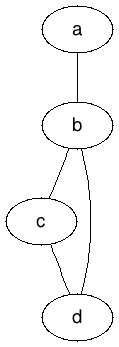
\includegraphics[width=2cm]{images/input_graph.png} 
\caption[Graph]{Input graph}
\label{fig:arbitrary-graph}
\end{subfigure}
\begin{subfigure}[b]{\linewidth}
\centering
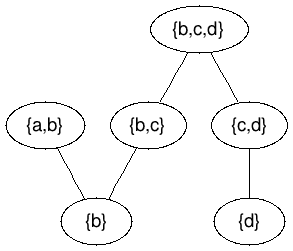
\includegraphics[width=6cm]{images/nice_tree_decomp.png} 
\caption[Decomposition]{Nice tree decomposition of the graph in figure \ref{fig:arbitrary-graph} of width $|\left\{b, c, d\right\}| - 1 = 2$. The root node is $\left\{ d \right\}$.}
\label{fig:decomp-graph}
\end{subfigure}
\end{figure}

\section{Counting homomorphisms}
\label{section:injhomo}
One approach to counting isomorphic subgraphs is to consider maps of $P$ onto subgraphs of $H$, and count the number of injective maps.
Formally we have the following:

\begin{defn}
A \emph{homomorphism} is a map $\phi : V(P) \rightarrow V(H)$ that preserves structure,
i.e. $\left\{v_1, v_2\right\} \in E(P) \Rightarrow \left\{\phi(v_1), \phi(v_2)\right\} \in E(H)$.
\end{defn}

An \emph{injective homomorphism} is an injective such map and it is \emph{partial} if only a subset of the vertices is included.
It is useful to extend a partial injective homomorphism by mapping additional vertices while preserving the edge structure.
This might result in an extension that is no longer injective.

Let $hom_{\phi}(P, H)$ denote the number of homomorphisms extending some injective homomorphism $\phi$.
D{\'{\i}}az~{\em et al.}~\cite{DST02} introduced an algorithm for computing $hom_{\phi}(P, H)$ in time $O^*(|H|^{t_w(P)})$.
The paper uses the term \emph{list-colorings} and requires an existing nice tree decomposition of the pattern graph, which can be computed in polynomial time in the case of bounded treewidth.
In addition, the tree needs to be processed in a certain sequence as given in the following definition.

\begin{defn}
A \emph{stingy ordering} is an ordering $v_1, v_2, ..., v_{|T|}$ of all vertices in $V(T)$ s.t.:
\begin{itemize}
\item $v_1$ is a child node and $v_{|T|}$ is the root node
\item all parents of a node $v_i$ occur at indices $>i$ in the ordering
\end{itemize}
\end{defn}

The paper defines an additional criteria which ensures certain space bounds, but is left out of here for simplicity.
A Stingy ordering can be computed by performing a traversal of the input tree from the leafs to the root node.

Let $P_p = P[\cup_{v \in V(T_p)} X_v]$ be an induced subgraph for some pattern graph tree decomposition $(T, r, X)$, where $T_p$ denotes the subtree rooted in vertex $p$.
Algorithm \ref{count-homomorphisms} counts the number of homomorphisms extending some existing injective homomorphism $\phi$.
The outline corresponds to the one given in D{\'{\i}}az~{\em et al.}~\cite{DST02} as counting list-colorings, but only constrains any vertices in $\phi$ to their given target vertex.
Note that $F_p = \left\{X_p \rightarrow V(H)\right\}$, i.e. the set of all maps from the bag to the host graph.
In addition, $I_p(\psi)$ is the number of homomorphisms from $P_p$ onto $H$ that agree with $\psi$ on all vertices in $X_p$.

\begin{algorithm}
\begin{algorithmic}
\caption{Algorithm counting the number of homomorphisms extending an existing map}
\label{count-homomorphisms}
\Procedure{CountHomomorphisms}{$P, (T, r, X), H,\phi$}

\State $\texttt{S} \gets \Call{GenerateStingyOrdering}{T}$

\ForAll{$p \in S$} 
  \State $C \gets \texttt{children nodes of p in T}$
  \If {$C = \emptyset$ $\texttt{and}$ $X_p = \left\{ v \right\}$}
    \If {$v \in \phi$}
        \State $I_p((v, \phi(v))) \gets 1$
    \Else
        \State $\forall a \in V(H): I_p((v, a)) \gets 1$
    \EndIf
  \ElsIf {$C = \left\{q_1, q_2\right\}$}
      \State $\forall \psi \in F_p: I_p(\psi) \gets I_{q_1}(\psi) I_{q_2}(\psi)$
  \ElsIf {$C = \left\{q\right\}$ $\texttt{and}$ $X_p \setminus X_q \not = \emptyset $}
      \State $\left\{v\right\}\gets X_p \setminus X_q$
      \ForAll{$\psi \in F_q$ $\texttt{and}$ $a \in V(H)$} 
        \If {$\forall_{u \in S_q} \left\{\psi(u), a \right\} \in E(H)$}
            \State $I_p(\psi \cup \left\{v, a \right\}) \gets I_q(\psi)$
        \Else
            \State $I_p(\psi \cup \left\{v, a \right\}) \gets 0$
        \EndIf
      \EndFor
  \ElsIf {$C = \left\{q\right\}$ $\texttt{and}$ $X_q \setminus X_p \not = \emptyset $}
      \State $\left\{v\right\}\gets X_q \setminus X_p$
      \State $\forall \psi \in F_p: I_p(\psi) \gets \sum_{a \in V(H)} I_{q}(\psi \cup \left\{ (v,a) \right\})$
  \EndIf
\EndFor

\Return $I_r(\emptyset)$
\EndProcedure
\end{algorithmic}
\end{algorithm}

In order to retrieve partial results for the number of injective homomorphisms $inj_{\phi}(P, H)$ it is possible to apply inclusion-exclusion, as in a theorem due to Fomin \emph{et al.}~\cite{FLRRS12}:

\begin{thm}
\label{thm:fomin}
Given some $S \subseteq V(P)$ and an injective homomorphism $\phi : S \rightarrow V(H)$ then $inj_{\phi}(P, H[S' \cup \phi(S)])$
can be computed in time $O^*((\sum_{j=1}^{|P|-|S|}\binom{|H|}{j})|H|^{w_t(P)})$,
for all $S' \subseteq V(H) \setminus \phi(S)$ of size $|P| - |S|$.
\end{thm}

This result can be used as a subroutine when counting the total number of injective homomorphisms.
The actual calculation relies on the following equality ~\cite{FLRRS12}:

\begin{equation}
inj_{\phi}(P, H[S' \cup \phi(S)]) = \sum_{X \subseteq S'} (-1)^{|S'|-|X|} hom_\phi(P, H[X \cup \phi(S)])
\end{equation}

The time complexity follows by evaluating the LHS summand over all possible subsets $X$ (drawn from the universe), and aggregating the results to all $S'$ by using the trimmed zeta transform, as detailed in the paper.

Finally, the number of isomorphic subgraphs can be evaluated by calculating the number of injective homomorphisms from $P$ onto subgraphs of $H$, divided by the number of automorphisms on the pattern graph.
This can be expressed as $\textsc{IsoSubgraphs}(P, H) = \frac{inj(P, H)}{aut(P)} = \frac{inj(P, H)}{inj(P, P)}$ \cite{FLRRS12}.

\section{Thin subgraphs as weighted disjoint triples}
Using the notions introduced up to now, it is possible to study the contributions made by Bj\"orklund \emph{et al.}~\cite{BHKK13}.
The paper introduces the following function:

\begin{defn}
\label{def:delta}
$\Delta(f, g, h) = \sum_{\substack{A, B, C \in U\\A \cap B = A \cap C = B \cap C = \emptyset}} f(A)g(B)h(C)$
\end{defn}

This is used to express counting subgraphs in terms of algebraic objects. $U$ is a universe from which the three disjoint sets are drawn.
Similarly to a counting algorithm presented by Fomin~\emph{et al.}~\cite{FLRRS12}, Bj\"orklund \emph{et al.}~\cite{BHKK13} use a partition scheme which counts all injective isomorphisms in parts.

\begin{defn}
A \emph{balanced 3-way separation} of the pattern graph $P$ with bounded pathwidth $p$ is a collection of sets $L \sqcup S \sqcup M \sqcup T \sqcup R = V(P)$, such that:
\begin{itemize}
\item Every edge $e \in E(P)$ connects vertices between at most two consecutive sets in the ordering $L, S, M, T, R$.
\item The separator sets $S$ and $T$ have size bounded in the pathwidth, i.e. $|S|, |T| \leq p$
\item The remaining sets have $|L|, |M|, |R| \leq \frac{|P|}{3}$
\end{itemize}
\end{defn}

It can be constructed in polynomial time \cite{BHKK13}.

Now consider creating an injective homomorphism $\phi$ mapping $S$ and $T$ onto $H$, as visualized in the figure \ref{fig:homo-viz},
where $A,B,C \subseteq (H \setminus \phi(S) \setminus \phi(T))$.

\begin{figure}[here]
\centering
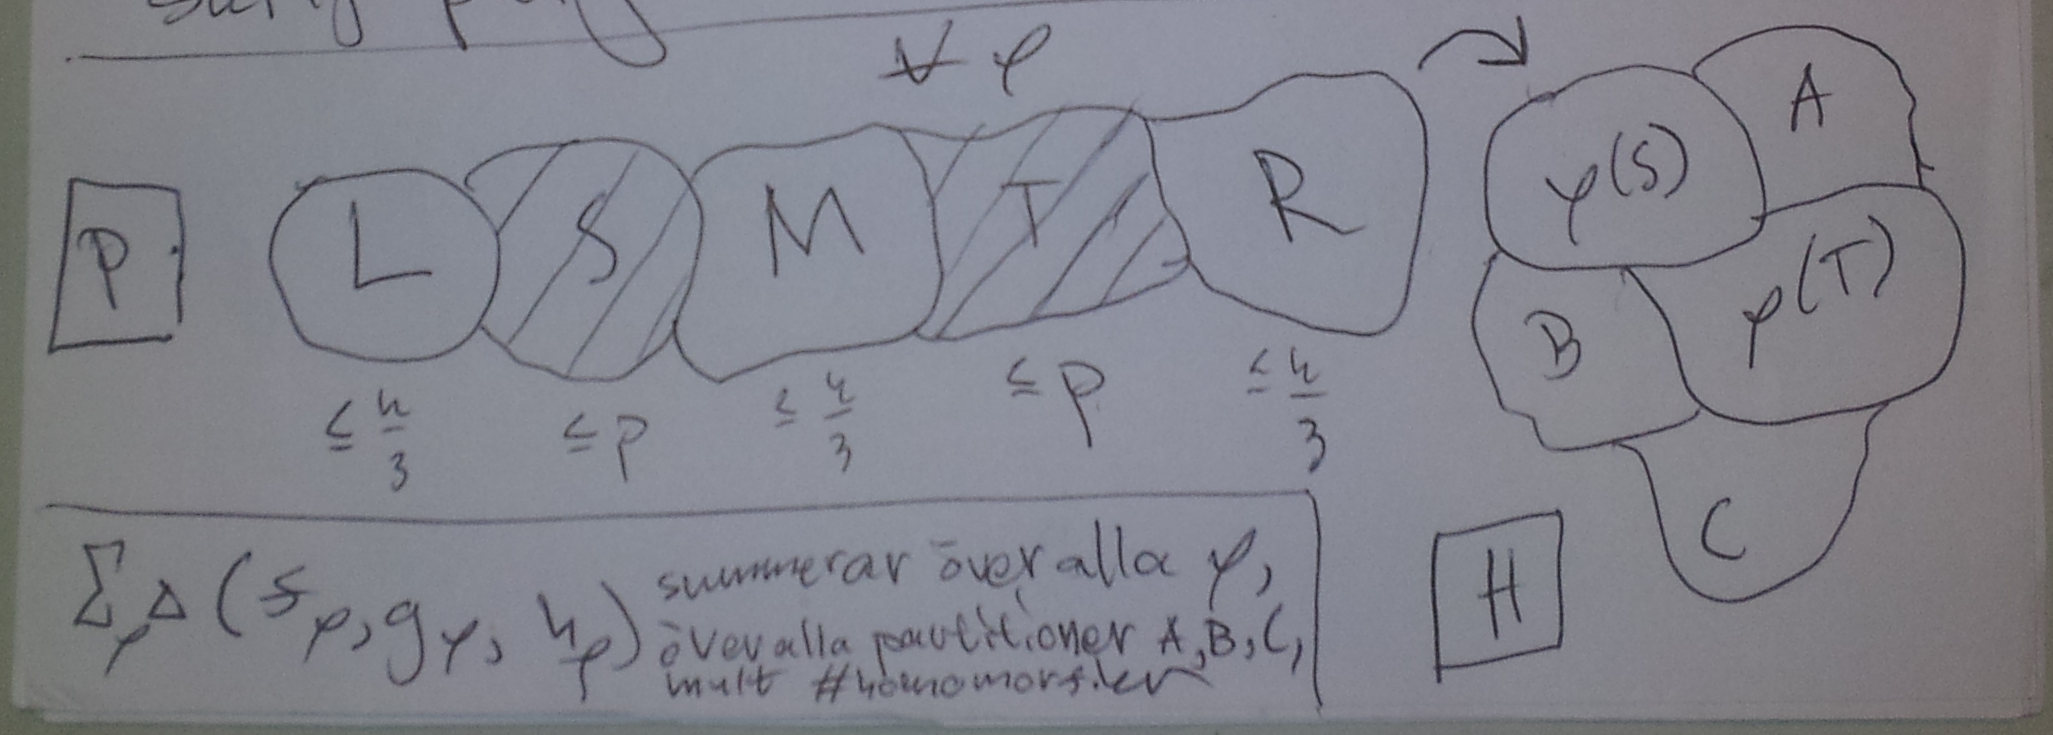
\includegraphics[width=8cm]{images/sketch_homo.png} 
\caption[Mapping]{Mapping of pattern graph onto host graph given an injective homomorphism $\phi$}
\label{fig:homo-viz}
\end{figure}

Enumerating all such possible $O(|H|^{2p})$ injective homomorphisms mapping $S$ and $T$ to the host graph,
all possible extensions to $\phi$ can be considered using theorem \ref{thm:fomin}.
Recall that $inj_\phi(P, H)$ denotes the number of injective homomorphisms extending $\phi$ from $P$ onto $H$.
Formally the following functions over subsets of the host graph are defined, for each candidate $\phi$:

\begin{itemize}
\item $f_\phi(A) = inj_\phi(P[L \cup S], H[A \cup \phi(S)])$
\item $g_\phi(B) = inj_\phi(P[S \cup M \cup T], H[\phi(S) \cup B \cup \phi(T)])$
\item $h_\phi(C) = inj_\phi(P[R \cup T], H[C \cup \phi(T)])$
\end{itemize}

Hence the number of injective homomorphisms extending a candidate $\phi$ is $\Delta_\phi(f_\phi, g_\phi, h_\phi)$ \cite{BHKK13}.

\section{Efficient weighted disjoint triples}
In the previous section the problem of counting isomorphic subgraphs was expressed as evaluating weighted disjoint triples.
The main contribution of the new result \cite{BHKK13} relates to how these can be efficiently evaluated, after all of the
injective homomorphisms on certain subgraphs have been calculated.
In other words we would like to calculate $\Delta_\phi$ efficiently.

The approach taken by the paper is to formulate the problem in terms of a linear equation system which can be constructed and solved within the runtime bound.
Hence the first step is to formulate a set of indeterminates to solve for.
Note that, for $q$-sized subsets $A,B,C \subseteq U$, it holds that $|A\oplus B\oplus C|\equiv |A|+|B|+|C|=3q\equiv q\pmod 2\,$ \cite{BHKK13}, where $\oplus$ denotes symmetric difference.
This implies that the symmetric difference is either odd or even, depending on $q$.
It follows that there are a total of $\lfloor \frac{3q}{2} \rfloor$ indeterminates on the following form (where $j \in \left\{ i \in [3q] | i \equiv_2 q \right\}$:

\begin{defn}
$x_j=x_j(f_\phi,g_\phi,h_\phi)=\sum_{\substack{A,B,C\in\binom{U}{q}\\|A\oplus B\oplus C|=j}}
f_{\phi}(A)g_{\phi}(B)h_{\phi}(C)\,.$
\end{defn}

Solving for $x_{3q}$ results in $\Delta_\phi$, since the size of the symmetric difference is maximized when all three subsets are disjoint \cite{BHKK13}. 

Given these indeterminates, the paper uses two different types of equations which combined together yield the final linear equation system.
The first family of equations is known as \emph{basic}:

\begin{defn}
A \emph{basic} equation for some $i$ is:

\begin{equation}
\label{eq:yi}
y_i=
\sum_{(u_1,u_2,\ldots,u_i)\in U^i}
T_0\bigl(\oplus_{\ell=1}^i\{u_\ell\}\bigr)
-T_1\bigl(\oplus_{\ell=1}^i\{u_\ell\}\bigr)\,.
\end{equation}

where

\begin{equation}
T_p(Z)=
\sum_{\substack{A,B,C\in\binom{U}{q}\\|(A\oplus B\oplus C)\cap Z|\equiv p\!\!\!\pmod 2}}
f_\phi(A)g_\phi(B)h_\phi(C)\,.
\end{equation}
\end{defn}

Combined with coefficients from a \emph{Vandermonde matrix}, given by $v_{ij} = (n - 2j)^i$, Bj\"orklund \emph{et al.}~\cite{BHKK13} prove that $\sum_j v_{ij}x_{j} = y_i$ holds.

The second family of equations is the following:

\begin{defn}
A \emph{simple} equation is the following, which holds for all indeterminates $x_j$:

\begin{equation}
\label{eq:xj-direct}
x_j
=
\sum_{\substack{\ell=q-j\\\ell\equiv 0\!\!\!\!\!\pmod 2}}^{q+j}
\sum_{D\in\binom{U}{\ell}}
\sum_{\substack{A,B\in\binom{U}{q}\\A\oplus B=D}}
f_\phi(A)g_\phi(B)
\sum_{\substack{C\in\binom{U}{q}\\|C\cap D|=(q+\ell-j)/2}}h_\phi(C)\,.
\end{equation}

\end{defn}

Given a parameter $0 \leq \gamma \leq 1/2$ the authors take the following:
\begin{itemize}
\item $\lfloor (3/2 - \gamma)q \rfloor$ simple equations solving for $x_j$
\item a number of basic equations, reaching the required number of independent equations
\end{itemize}

The parameter $\gamma$ is chosen in order to balance the contribution in running time from both of the families, which depends on the efficiency of evaluating certain matrix multiplications.
Assuming efficient evaluation of square matrix multiplication and multiplication of $N^\alpha \times N$ with an $N \times N^\alpha$ matrix, this results in time complexity $O^*(n^{0.4547|P|})$ in order to construct the system \cite{BHKK13}.

Following this, Gaussian elimination is applied on the system in order to solve the resulting set of equations in polynomial time, and return $x_{3q}$ as $\Delta_\phi$.

The procedure outlined above will be executed for all $O(|H|^{2p})$ injective homomorphisms $\phi$.
Summing over all $\Delta_\phi$ and dividing by the number of automorphisms gives the final number of isomorphic subgraphs.
Hence the final running time for counting thin subgraphs is $O^*(n^{0.4547|P| + 2p})$.

\chapter{Implementation}
This chapter describes an implementation of \emph{counting thin subgraphs} \cite{BHKK13}.
The implementation is available as a git repository \footnote{\url{https://github.com/davnils/count-subgraphs}}.

\section{Overview}
Counting of thin subgraphs has been implemented as presented in the paper \cite{BHKK13} with some implementation differences.
Internally it generates tree decompositions using the routine \emph{create\_join\_tree} available in the library dlib 18.5 \footnote{\url{http://www.dlib.net}}
Nice tree decompositions \cite{kintali12} and counting homomorphisms \cite{DST02} have been implemented as described in the corresponding papers.
The space bounds mentioned as a third criteria in stingy orderings have been ignored since there practical cost is not an issue, at least with the relevant graph sizes.

Counting injective homomorphisms \cite{FLRRS12} has been implemented partially as described.
As mentioned in section \ref{section:injhomo}, the number of homomorphisms over all subsets is evaluated.
The aggregation is however done naively without using the zeta transform, incurring additional work.

Pattern partitioning has been implemented as an exhaustive search supporting different acceptance criteria, supplied as a predicate over the resulting sets ($L, S, M, T, R$).
Counting isomorphic subgraphs involves partitioning the pattern graph such that $S$ and $T$ are non-empty, and $L, M, R$ are of equal size.
The motivation for restricting the implementation to equally sized subsets is that the paper describes processing $q$-sized subsets from the universe, but this might be possible to generalize.

Basic and simple equations have also been implemented, as specified \cite{BHKK13}.
There is one trade-off where the intersection transform is calculated by enumerating all subsets instead of relying on evaluation through arithmetic circuits~\cite{BHKK08}.
The linear system is built from any solved indeterminates, gathered from simple equations, and is combined with basic equations.
It is solved by performing LU-decomposition using routines available in the boost library \footnote{\url{http://www.boost.org}}.

\section{Correctness}
Correctness verification has been performed by building a test suite.
All implemented components have separate test cases which attempt to evaluate correctness within the available computational resources.
One common way of verifying the implemented algorithms has been to implement the corresponding naive versions.
These have been evaluated over random graphs of different sizes, including boundary instances such as single vertices.
An example of this includes counting (optionally injective) homomorphisms by performing an exhaustive search.
This is implemented by extending an existing homomorphism with an additional vertex in each step, and moving to the next candidate vertex.

\section{Performance}
Part of this project involved studying the implementation from a performance perspective, and building benchmarks testing the performance.
The performance is however very limited and the implementation is not usable in real-life scenarios.
It is possible to count subgraph isomorphisms on randomized pattern and host graphs up to about 10 vertices each in a time frame of seconds.

The implementation is structured into two phases: generation of triples containing injective homomorphism counts between subgraphs, and building of linear equation systems.
Each injective homomorphism mapping the partitions $S$ and $T$ onto the subgraph is considered in isolation.
The runtime of the first phase is heavily dependent on the number of such candidates, but also on the underlying graphs being considered.
This follows since all possible extensions are considered until the whole pattern graph is mapped onto the host graph.

The runtime of the second phase is mostly dependent on the number of candidate injective homomorphisms.
Each candidate generates a linear equation system but the generation is not a considerable bottleneck with the restrictive graph sizes.

\section{Conclusion}
This report has explained the counting thin subgraphs algorithm and the underlying subroutines needed in order to implement it.
The recent algorithmic advances are of interest primarily due to the meet-in-middle barrier being broken in terms of time complexity.

An implementation has been made of the algorithm in order to provide a deeper understanding of the results and survey real-life performance.
The specific implementation is not very useful in real-life settings due to being limited to relatively small graphs.
One practical issue with implementing these algorithms is generating tree decompositions which is considered to be in polynomial time for fixed treewidth, but still has big constants for optimal solutions.

An alternative to implementing the more complex algorithms for counting subgraphs is to rely on exhaustive searches.
This is likely to perform well when combined with efficient heuristics, but also provides a good starting point in terms of a simple implementation suitable for quick evaluation.
In addition this does not constrain input graphs to have specific structural properties in order to reach the specified asymptotic bounds.

\begin{thebibliography}{10}

\bibitem{BHKK13}
A.~Bj{\"o}rklund, P.~Kaski, and L.~Kowalik.
\newblock Counting Thin Subgraphs via Packings Faster Than Meet-in-the-Middle Time.
\newblock {\em Proc. of the 25th Annual ACM-SIAM Symp. on Disc. Algo.}  45:594--603, 2014.

\bibitem{B10}
A.~Bj{\"o}rklund.
\newblock Determinant Sums for Undirected Hamiltonicity
\newblock {\em Prof. of FOCS’10, 2010}  173--182, 2010.

\bibitem{FG06}
J.~Flum, and M.~Grohe.
\newblock Parameterized complexity theory.  Vol. 3.
\newblock Heidelberg: Springer, 2006.

\bibitem{FG04}
J.~Flum, and M.~Grohe.
\newblock The parameterized complexity of counting problems.
\newblock {\em SIAM J. Comput.}, 33(4):892--922, 2004.

\bibitem{ARORA96}
S.~Arora.
\newblock Polynomial time approximation schemes for Euclidean TSP and other geometric problems.
\newblock {\em Foundations of Computer Science, 1996. Pro., 37th ann. sym.} (pp. 2-11). IEEE. 1996.

\bibitem{DELL10}
H.~Dell, and D.~van Melkebeek.
\newblock Satisfiability allows no nontrivial sparsification unless the polynomial-time hierarchy collapses.
\newblock {\em Proceedings of the 42nd ACM symposium on Theory of computing} (pp. 251-260). ACM. 2010.

\bibitem{KOBLER94}
J.~Köbler, U.~Schöning, and J.~Torán.
\newblock The graph isomorphism problem: its structural complexity.
\newblock Birkhauser Verlag. 1994.

\bibitem{W09}
R.~Williams.
\newblock Finding Paths of Length $k$ in $O^*(2^k)$ Time.
\newblock {\em Inform. Process. Lett.} 109(6) pp.~315--318, 2009.

\bibitem{VW09}
V.~Vassilevska and R.~Williams.
\newblock Finding, minimizing, and counting weighted subgraphs.
\newblock In M.~Mitzenmacher, editor, {\em STOC}, pages 455--464. ACM, 2009.

\bibitem{DST02}
J.~D{\'{\i}}az, M.~Serna, and D.~M. Thilikos.
\newblock Counting {$H$}-colorings of partial {$k$}-trees.
\newblock {\em Theoret. Comput. Sci.}, 281(1-2):291--309, 2002.
\newblock Selected papers in honour of Maurice Nivat.

\bibitem{FLRRS12}
F.~V. Fomin, D.~Lokshtanov, V.~Raman, S.~Saurabh, and B.~V.~R. Rao.
\newblock Faster algorithms for finding and counting subgraphs.
\newblock {\em J. Comput. Syst. Sci.}, 78(3):698--706, 2012.

\bibitem{bodlaender96}
H. L.~Bodlaender.
\newblock A linear-time algorithm for finding tree-decompositions of small treewidth.
\newblock {\em SIAM Journal on computing}, 25(6), 1305-1317, 1996.

\bibitem{ergun02}
F.~Ergun, R.~Sinha, and L.~Zhang.
\newblock An improved FPTAS for restricted shortest path.
\newblock {\em Information Processing Letters}, 83(5), 287-291, 2002.

\bibitem{kintali12}
S.~Kintali, and S.~Munteanu.
\newblock Computing Bounded Path Decompositions in Logspace.
\newblock {\em Electronic Colloquium on Computational Complexity (ECCC)}, 19:126, 2012.

\bibitem{carr00}
H.~Carr, J.~Snoeyink, and U.~Axen.
\newblock Computing contour trees in all dimensions.
\newblock {\em Proceedings of the eleventh annual ACM-SIAM symposium on Discrete algorithms}, pp. 918-926. (2000).

\bibitem{BHKK08}
A.~Bj{\"o}rklund, T.~Husfeldt, P.~Kaski, and M.~Koivisto.
\newblock The fast intersection transform with applications to counting paths.
\newblock {\em CoRR}, abs/0809.2489, 2008.

\end{thebibliography}

\end{document}
